% -----------------------------------------------
% Template for ICMC SMC 2014
% adapted and corrected from the template for SMC 2013,  which was adapted from that of  SMC 2012, which was adapted from that of SMC 2011
% -----------------------------------------------

\documentclass{article}
\usepackage{icmcsmc2014}
\usepackage{times}
\usepackage{ifpdf}
\usepackage[english]{babel}

% TL: Custom package so that multi-line maths equations can be properly aligned
\usepackage{amsmath}

% TL: Custom package so that distance between figures and captions can be reduced when needed.
\usepackage{caption}

% JA: Custom packages for Wide figures in two column documents
% See: http://en.wikibooks.org/wiki/LaTeX/Floats,_Figures_and_Captions
\usepackage{dblfloatfix}
\usepackage{fixltx2e}

%\usepackage{cite}

% Multipart figures
%\usepackage{subfigure}

% Surround parts of graphics with box
%\usepackage{boxedminipage}

%%%%%%%%%%%%%%%%%%%%%%%% Some useful packages %%%%%%%%%%%%%%%%%%%%%%%%%%%%%%%
%%%%%%%%%%%%%%%%%%%%%%%% See related documentation %%%%%%%%%%%%%%%%%%%%%%%%%%
%\usepackage{amsmath} % popular packages from Am. Math. Soc. Please use the 
%\usepackage{amssymb} % related math environments (split, subequation, cases,
%\usepackage{amsfonts}% multline, etc.)
%\usepackage{bm}      % Bold Math package, defines the command \bf{}
%\usepackage{paralist}% extended list environments
%%subfig.sty is the modern replacement for subfigure.sty. However, subfig.sty 
%%requires and automatically loads caption.sty which overrides class handling 
%%of captions. To prevent this problem, preload caption.sty with caption=false 
%\usepackage[caption=false]{caption}
%\usepackage[font=footnotesize]{subfig}


%user defined variables
\def\papertitle{ATK Reaper: Ambisonic Toolkit as JSFX plugins}
\def\firstauthor{Trond Lossius}
\def\secondauthor{Joseph Anderson}
%\def\thirdauthor{Third author}

% adds the automatic
% Saves a lot of ouptut space in PDF... after conversion with the distiller
% Delete if you cannot get PS fonts working on your system.

% pdf-tex settings: detect automatically if run by latex or pdflatex
\newif\ifpdf
\ifx\pdfoutput\relax
\else
   \ifcase\pdfoutput
      \pdffalse
   \else
      \pdftrue
\fi

\ifpdf % compiling with pdflatex
  \usepackage[pdftex,
    pdftitle={\papertitle},
    pdfauthor={\firstauthor, \secondauthor},
    % pdfauthor={\firstauthor, , \thirdauthor},
    bookmarksnumbered, % use section numbers with bookmarks
    pdfstartview=XYZ % start with zoom=100% instead of full screen; 
                     % especially useful if working with a big screen :-)
   ]{hyperref}
  %\pdfcompresslevel=9

  \usepackage[pdftex]{graphicx}
  % declare the path(s) where your graphic files are and their extensions so 
  %you won't have to specify these with every instance of \includegraphics
  \graphicspath{{./figures/}}
  \DeclareGraphicsExtensions{.pdf, .jpeg, .png}


  \usepackage[figure,table]{hypcap}

\else % compiling with latex
  \usepackage[dvips,
    bookmarksnumbered, % use section numbers with bookmarks
    pdfstartview=XYZ % start with zoom=100% instead of full screen
  ]{hyperref}  % hyperrefs are active in the pdf file after conversion

  \usepackage[dvips]{epsfig,graphicx}
  % declare the path(s) where your graphic files are and their extensions so 
  %you won't have to specify these with every instance of \includegraphics
  \graphicspath{{./figures/}}
  \DeclareGraphicsExtensions{.eps}

  \usepackage[figure,table]{hypcap}
\fi

%setup the hyperref package - make the links black without a surrounding frame
\hypersetup{
    colorlinks,%
    citecolor=black,%
    filecolor=black,%
    linkcolor=black,%
    urlcolor=black
}


% Title.
% ------
\title{\papertitle}

% Authors
% Please note that submissions are NOT anonymous, therefore 
% authors' names have to be VISIBLE in your manuscript. 
%
% Single address
% To use with only one author or several with the same address
% ---------------
% \oneauthor
%    {\firstauthor} {BEK - Bergen Centre for Electronic Arts \\ %
%      {\tt \href{mailto:trond.lossius@bek.no}{trond.lossius@bek.no}}}

%Two addresses
%--------------
\twoauthors
  	{\firstauthor} {BEK - Bergen Centre for Electronic Arts\\ %
	  {\tt \href{mailto:trond.lossius@bek.no}{trond.lossius@bek.no}}}
    {\secondauthor} {DXARTS, University of Washington \\ %
      {\tt \href{joanders@uw.edu}{joanders@uw.edu}}}

% Three addresses
% --------------
% \threeauthors
%   {\firstauthor} {Affiliation1 \\ %
%     {\tt \href{mailto:author1@smcnetwork.org}{author1@smcnetwork.org}}}
%   {\secondauthor} {Affiliation2 \\ %
%     {\tt \href{mailto:author2@smcnetwork.org}{author2@smcnetwork.org}}}
%   {\thirdauthor} { Affiliation3 \\ %
%     {\tt \href{mailto:author3@smcnetwork.org}{author3@smcnetwork.org}}}


% ***************************************** the document starts here ***************

\begin{document}
%
\capstartfalse
\maketitle
\capstarttrue




%%%%%%%%%%%%%%%%%%%%%%%%%%%%%%%%%%%%%%%%%%%%%%%%%%%%%%%%%%%%%%%%%%%%%%%%%%%%%
% Abstract
%%%%%%%%%%%%%%%%%%%%%%%%%%%%%%%%%%%%%%%%%%%%%%%%%%%%%%%%%%%%%%%%%%%%%%%%%%%%%
\begin{abstract}
While there is a well-established workflow for stereo in DAWs, options have been more limited when working with Ambisonics.
The Ambisonic Toolkit (ATK) brings together a number of tools and transforms for working with First order Ambisonic surround sound, including intriguing possibilities for spatial transforms of soundfield image.
Previously these tools have only been available in the real-time processing environment SuperCollider.

Reaper is a reasonably priced and flexible DAW for spatial sound, popular among many composers and sonic art\-ists working with spatial sound.
ATK has been ported to plugins for the Cockos Reaper DAW using the JSFX text-based scripting language, with intuitive graphical user interfaces.
As compared to development in C++, this has simplified the effort, and plugins are immediately available for all platforms supported by Reaper.
Future maintenance is also expected to be less demanding.

%ATK is framed for the user to `think Ambisonically'. By this, it is meant the ATK is focused on the problem of synthesising and processing sound fields. And, the model of the ATK is a sound-field sound-image model rather than a sound-object sound-scene model. Now one can `think Ambisonically' in a DAW as well.
\end{abstract}




%%%%%%%%%%%%%%%%%%%%%%%%%%%%%%%%%%%%%%%%%%%%%%%%%%%%%%%%%%%%%%%%%%%%%%%%%%%%%
% Introduction
%%%%%%%%%%%%%%%%%%%%%%%%%%%%%%%%%%%%%%%%%%%%%%%%%%%%%%%%%%%%%%%%%%%%%%%%%%%%%
\section{Introduction}\label{sec:introduction}

\subsection{Spatial sound representations}\label{sec:spatial-sound}

Spatial sound is usually represented in one of three ways: as channel feeds, as spatial scene descriptions, or as sound field encodings.
ITU 5.1 and ITU 7.1 are examples of fixed-channel distribution formats \cite{ITU:1993_surround_5:1}.
This approach becomes less practical as the number of channels increases, and also has clear limitations due to the lack of flexibility in loudspeaker positioning.
Object-based spatial scene descriptions instead associate sound sources with meta-information describing location or direction. In this way an auditory scene can be described independently of loudspeaker setup, and rendered appropriately for a chosen playback system.
This is the approach used for e.g., Dolby Atmos and Wave Field Synthesis \cite{dolby:2014atmos,Berkhout:1993wfs}.
SpatDIF, the Spatial Sound Description Interchange Format, is an open format offering a semantic and syntactic specification for storing and transmitting such spatial audio scene descriptions \cite{Peters:2013spatdif}.

Ambisonics encodes audio sources into a speaker-inde\-pendent representation of the sound field called B-format  \cite{gerzon:1985JAES}.
Decoding is the process where an encoded sound field is translated to individual speaker channel feeds; an advantage being,  decoders can be designed for different speak\-er arrays.
Ambisonics is based on spherical harmonic decomposition of the sound field, and depending on truncation of the spherical harmonic decomposition, 
the B-for\-mat signal may be First order Ambisonic (FOA) or higher order (HOA)\footnote{Third order Ambisonic is often abbreviated TOA.} \cite{daniel:2001phd}.

Spatial resolution improves with increasing order, but so does the number of channels required for the encoded signal.
A number of commercial microphones are available for recording in FOA, and free or commercial B-format recordings are available as sound effects libraries \cite{farrar:1979soundfield,deleflie2014:ambisonia,darcourt:2014surlib}.




\subsection{Spatial sound processing in DAWs}\label{sec:daws}

Encoding, processing and decoding of B-format signals requires support for multi-channel signals.
Real-time programming environments are well-suited in this respect as they offer flexible configuration and routing of channels. Ambisonics is supported in all major real-time audio programming environments, such as Csound, Max, Pd and SuperCollider, often as 3rd party extensions to these programs.

The support for surround sound is more limited in most Digital Audio Workstation (DAW) programs.
Ableton Live is primarily geared towards stereo, although Max 4 Live devices can be used for spatialisation by routing signals to several buses.
Most DAWs that support surround sound, such as Adobe Audition, Cubase, Logic Pro X and Pro Tools are oriented towards fixed-channel distribution formats, with an upper limit of 6 (5.1) or 8 (7.1) channels.
% TODO: Very difficult to figure out what Ardour is capable of or not. On my Mac t's just crashing, but that's not very informative. I see some web sites claiming you can do quite a bit surround-sound-wise in Ardour, and others that says that it's mostly broken.
% Reference Adobe Audition: https://helpx.adobe.com/audition/using/5-1-surround-sound.html
Digital Performer also supports 10.2, and Nuendo supports up to 13 channels in various fixed-channel distribution formats.
Nuendo and Pro Tools can be extended to support object-based spatial scene descriptions.
The Iosono Spatial Audio Workstation program plug-in for Nuendo extends the capabilities of this program by adding abilities for object-based manipulation of sound sources \cite{iosono2012:workstation}, and can be used with Iosono Core hardware systems for wave-field synthesis.
% DISCUSS: Do we need to add references to the manuals for each of these programs, or is it sufficient to do it for the more specialised ones, such as Nueundo and IOSONO?
Dolby Atmos authoring is achieved using ProTools and the Dolby Rendering and Mastering Unit (RMU).
RMU provides the rendering engine for the mix stage, and integrates with Pro Tools through the Dolby Atmos Panner plug-in over Ethernet for metadata communication and monitoring. 
The metadata is stored in the Pro Tools session as plug-in automation \cite{dolby:2013authoring}.

The DAWs discussed so far are either limited with respect to surround sound abilities, or expensive and proprietary software and hardware systems for object-based spatial scene authoring and rendering.
In contrast Reaper is a reasonably priced and flexible DAW for spatial sound \cite{cockos:2014reaper}.
Reaper supports tracks of up to 64 channels\footnote{Suitable for 7\textsuperscript{th}-order HOA.}, and is exceptionally open-ended with respect to routing of channels and tracks.
Reaper supports all standard fixed-channel surround sound configurations, and the ReaSurround panning plugin that is integrated with Reaper also caters for non-standard speaker configurations \cite{francis:2014_reaper}, using a spatialisation algorithm based on principles resembling VBAP \cite{Pulkki:1997vbap} as well as DBAP \cite{Lossius:2009dbap}.
Reaper is well-suited for Ambisonics as well, and is a preferred DAW for many composers within the Ambisonic  community \cite{wiggins:2012reaperhowto}.

% TODO: ** FX processing chains in DAWs - as a motivation for why we want to be able to work the same way with Ambisonics, and make Ambisonic sound field recordings a malleable material in acousmatic mucis composition and sound design. Maybe this should be at the very start?




\subsection{Plugin technologies}\label{sec:plugin-technologies}

Several plugin specifications enable development of virtual instruments and effects that can be used with multiple hosts.
VST is a plugin interface specification and SDK for Windows, Mac OSX and Linux by Steinberg \cite{steinberg:2014vst}.
It is a popular format for commercial and freeware plugins, mostly using the VST 2 SDK, and a large number of audio applications support VST under license from its creator.
AudioUnits (AU) is a Mac OSX-specific plugin architecture provided by Apple as part of CoreAudio \cite{apple2014:au}.
In a similar way DirextX can be used for development of Windows-only plugins \cite{microsoft2014:directX}.
LADSPA is a GNU LGPL plugin architecture mostly used on the Linux platform \cite{furse:2007ladspa}, and is gradually superseded by LADSPA version 2 (LV2) \cite{lv2:2014}.

While the above formats can be used to develop plugins for use with multiple hosts, there are also a number of specifications that permits 3rd part development of plugins for one hosting environment only.
Avid has developed the RTAS, TDM and more recently AAX plugin format that work with their software and hardware exclusively.
Ableton and Cycling'74 jointly offer Max for Live, enabling the use of Max patches as devices in Ableton Live \cite{ableton:2014maxforlive}. JSFX is a text-based scripting language for programming audio-oriented effects compiled on the fly for Cockos Reaper \cite{cockos:2014jsfx,cockos:2014reaper}.

The multiple operation systems and plugin architectures poses challenges to plugin developers, that ideally might want to offer their software work with all plugin architectures and hosts in all operation systems.
Developing, compiling and maintaining plugins for many parallel platforms can introduce substantial workload overhead, and several cross-platform plugin development frameworks have been developed to address this, e.g.,  JUCE \cite{juce2014}, wdl-ol \cite{larkin2014wdl-ol} and FAUST \cite{smithFaust:2012}. 
\emph{SonicBirth} can be used to create AudioUnit and VST plugins for OSX and Windows by connecting objects in a graphical programming environment. Development stalled in 2007, but recent renewed efforts have resulted in a version 2 public alpha being available \cite{sonicbirth2014}.
\emph{SynthEdit} is a similar technology for VST plugin development on the Windows platform \cite{synthedit2011}.


\subsection{Plugins for Ambisonic processing}\label{sec:ambi-plugins}

In recent years a number of plugins have emerged for Ambisonic processing.
\emph{WigWare} is a set of VST plugins for Mac and Windows that includes FOA and HOA panner and decoders for regular and irregular speaker layouts, as well as a FOA 3D reverb \cite{Wiggins:2010wigware}.
Danielle Courville has developed a number of FOA plugins in SonicBirth for encoding and decoding, correcting misaligned B-Format streams, performing rotations, mixing, reverb, and decoding, as well as encoders and decoders for 2nd order and planar 5th order Ambisonic \cite{courville:2012b2x}.
Due to the long halt in development of SonicBirth, these plugins do not work reliable in all newer versions of DAW programs.
\emph{ambiX} are cross-platform 1st, 3rd and 5th order Ambisonic processors for encoding and decoding, including binaural decoding, as well as spatial transforms \cite{Kronlachner2013:ambix,Kronlachner:2014ambi-transforms}.
These plugins use the ambiX encoded signal convention; full 3D, ACN channel ordering and SN3D normalization \cite{Nachbar:2011ambix} as discussed in section~\ref{sec:coordinate-systems}, but also provides a plugin for conversions to other formats.
They are accompanied by \emph{mcfx}, a number of more general multichannel plugins for equalising, delay, gain adjustment and level metering \cite{kronlachner2014:mcfx}.
\emph{Flux Ircam Spat} wraps the Ircam Spatialisateur multiformat room acoustics simulation and localization software as AU and VST plugins for Mac and Windows \cite{flux:2010spat}.
Although this plugin mainly provides object-based scene descriptions, it can render the auralization as B-format.
The \emph{HARPEX} plugin for decoding FOA uses an algorithm based on high angular resolution planewave expansion (HARPEX) in order to address issues with low angular resolution and small sweet spot that FOA suffers from \cite{Berge:2010harpex}.
Blue Ripple Sound offers a wide range of OSX and Windows VST plugins for TOA, including encoders and upmixers, decoders, and a rich set of plugins for spatial and filter-based manipulations of the encoded signal.
The TOA Harpex Upsampler converts FOA material to TOA using the Harpex algorithm \cite{blueripple:2014TOA}.




%%%%%%%%%%%%%%%%%%%%%%%%%%%%%%%%%%%%%%%%%%%%%%%%%%%%%%%%%%%%%%%%%%%%%%%%%%%%%
% ATK
%%%%%%%%%%%%%%%%%%%%%%%%%%%%%%%%%%%%%%%%%%%%%%%%%%%%%%%%%%%%%%%%%%%%%%%%%%%%%
\section{Ambisonic Toolkit}\label{sec:atk}

\begin{figure*}[t]
\captionsetup{aboveskip=-6pt}
\centering
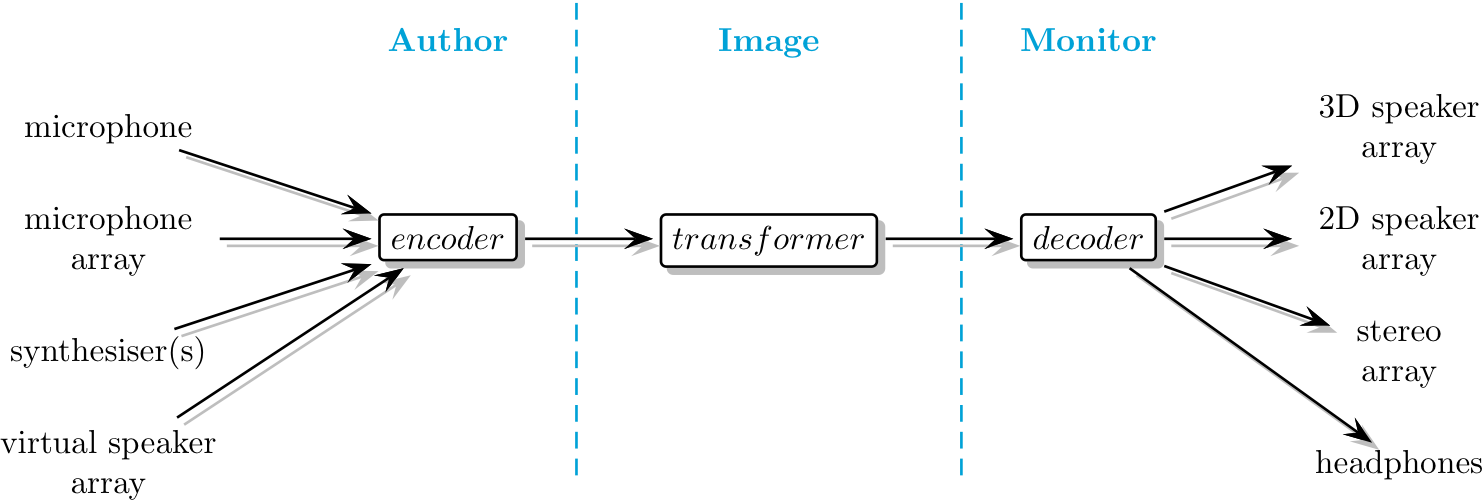
\includegraphics[width=2.0\columnwidth]{figures/atk-network.png}
\setlength{\abovecaptionskip}{0pt plus 3pt minus 2pt} % Decrease distance, as the figure itself has lots of empty space below
\caption{Ambisonic Toolkit Paradigm.\label{fig:atkParadigm}}
\end{figure*}

The Ambisonic Toolkit (ATK) brings together a number of tools and transforms for working with Ambisonic surround sound  \cite{Anderson:2009introducingATK, anderson:ambisonic_2011}.
Use is targeted towards the composer of acousmatic and experimental music. The intention is for the toolset to be both ergonomic and comprehensive, providing algorithms to creatively manipulate and synthesize Ambisonic sound fields.

The tools are framed for the user to `think Ambisonically'. By this, it is meant the ATK is focused on the problem of synthesising and processing sound fields. The model of the ATK is a sound-field sound-image model rather than a sound-object sound-scene model. By addressing the holistic problem of creatively controlling a complete soundfield, the ATK allows and encourages the composer to think beyond the placement of sounds in a sound-space and instead attend to the impression and image of a soundfield. This is viewed to be the {\em idiomatic} approach for working with the Ambisonic technique, and creatively leverages the model the Ambisonic technology presents.


%By this, it is meant the ATK is not focused on the problem of auralization and/or room modelling.
%Auralization is a complex problem beyond the scope of the fundamental algorithms of the ATK.
%It is worth noting, however, with the toolset provided, successful room modelling may be implemented.
%Interestingly enough, many composers of acousmatic music often do not move beyond the problem of auralization or room modelling.


Since 1998 the ATK has existed in a variety of forms.
In its very first implementation, the ATK was deployed as a collection of Csound orchestras, and a collection of VST plugins have previously been distributed.
% TODO: Should this be added?
% From 2007, an implementation for the Common Lisp Music(external link) synthesis and signal processing package has been under development.
Development of the real-time ATK library for SuperCollider2 began in 2000, and in recent years ATK has primarily been distributed as a version for SuperCollider3 \cite{Anderson:2009introducingATK}.
Some of the underlying ideas of ATK has also been incorporated into the Blue Ripple Sound Third order Ambisonic plugins \cite{blueripple:2014TOA}.
% TODO: Mention the adaptation of B<->A in Blue Ripple TOA

%TODO: ADD ATK paradigm discussion -- break this into several labelled sections. Refer to illustration.
%            Author --> Image --> Monitor
\subsection{Ambisonic Toolkit Paradigm}\label{sec:atk-model}



Figure \ref{fig:atkParadigm} illustrates how the ATK separates the task of production work with Ambisonics into three distinct elements:

\begin{description}
  \item[Author:] Capture or synthesise an Ambisonic soundfield.
  \item[Image:] Spatially filter an Ambisonic soundfield.
  \item[Monitor:] Playback or render an Ambisonic soundfield.
\end{description}

In its most simple form, Ambisonics can be regarded as splitting the panning law into two separate parts, {\em encoding} and {\em decoding}, where final panning ({\em decoding}) is deferred to an actual loudspeaker array at the time of playback. Many currently available implementations of Ambisonics take this approach. However, while giving much flexibility, especially for final playback, this view doesn't completely leverage the sound-field sound-image model made available in Ambisonics. The ATK considers intervention in {\em imaging} to be an critical step; this is where the artist shapes and processes the sound field in a coherent way which isn't easily available via the other models for working with spatial sound.

Further details are discussed in section~\ref{sec:implementation}, below.


%%%%%%%%%%%%%%%%%%%%%%%%%%%%%%%%%%%%%%%%%%%%%%%%%%%%%%%%%%%%%%%%%%%%%%%%%%%%%
% Design considerations
%%%%%%%%%%%%%%%%%%%%%%%%%%%%%%%%%%%%%%%%%%%%%%%%%%%%%%%%%%%%%%%%%%%%%%%%%%%%%
\section{ATK Reaper: Design considerations}\label{sec:design}

\subsection{Coordinate systems and encoding conventions}\label{sec:coordinate-systems}

Within the spatial audio community several coordinate system conventions are being used in parallel.
Theory on Ambisonic generally assume the same coordinate system conventions as acoustics, with the $x$-axis pointing forward, $y$-axis to the left, and the $z$-axis pointing upwards. 
Spherical coordinates also follows standard mathematical conventions, with $0^{\circ}$ azimuth being forward, and angles increasing in the anti-clockwise direction so that $90^{\circ}$ azimuth is to the left.
Positive elevation is upwards.
This is the coordinate system convention used by ATK for SuperCollider

SpatDIF use a navigation-based coordinate system with $x$-axis to the right and, $y$-axis pointing forward, and $z$-axis pointing upwards.
Azimuth is $0^{\circ}$ in the forward direction, and angles increase clockwise so that $90^{\circ}$ azimuth is to the right.
Positive elevation is upwards \cite{Peters:2013spatdif}.

There are also several conventions for how encoded Ambisonic signals are represented.
B-format recordings made with one type of encoding and played back using another will have severe mismatches in amplitude levels and channel order.

Classical \emph{Furse-Malham} encoding can be used for up to third-order signals, and seem to be the preferred representation in musical applications.
First order Furse-Malham encoded signals adhere to acoustics coordinate conventions.
The $W$ component is the pressure (omni or mono) component of the signal, $W$ is the pressure gradient component in the forward-backwards direction, $Y$ is the pressure gradient component in the left-right direction (the stereo component of an MS signal) and $Z$ is the up-down pressure gradient component.
Furse-Malham encoding is the preferred format for all of the Ambisonic plugins discussed is section \ref{sec:ambi-plugins} except ambiX, and Ambisonic recordings done using SoundField microphones also use this format.

\emph{Normalised 3D formulas (N3D)} and \emph{semi-normalised 3D formulas (SN3D)} can be used for higher order encoding and decoding  \cite{daniel:2001phd}, also beyond TOA.
N3D component signals go beyond unity $(-1, 1)$ and can only be properly stored in sound file formats that supports floating-points, whereas SN3D component signals stay within unity. 

ATK for Reaper uses First order Furse-Malham encoded signals throughout.
This ensures interoperability between ATK for Reaper and other sources and processors of Ambisonic signals such as ATK for SuperCollider or recorded Ambisonic signals, as well as most other available plugins.

ATK for Reaper strives to provide a consistent and intuitive interface towards scene description parameters such as direction of sources, speakers and spatial transforms, regardless of whether the user is accustomed with acoustics or navigational coordinate systems.
For this reason Cartesian coordinates are avoided throughout the plugin suite, and whenever possible the plugins offers graphical user interfaces to avoid ambiguities.

However, due to current limitations in the Reaper JSFX API, there are some considerations to be made with respect to description of azimuths.
The desired behaviour is that azimuths increase anti-clockwise.
At the same time it is also preferable that for sources coming from the front half circle, moving the azimuth slider to the right results in the direction of the sound also moving clockwise to the right, similar to what happens when moving a regular stereo pan pot.
The Harpex and Blue Ripple plugins both functions this way.
In order to achieve this, horizontal azimuth sliders will need to implemented with increasing values to the left.
This is however currently not supported in Reaper JSFX, and for the time being ATK for Reaper uses azimuth values described according to a navigational coordinate system.
If Reaper in the future is updated to support sliders with increasing values to the left, this design decision is likely to be reconsidered, and changed to use acoustic conventions.




\subsection{Graphical user interfaces in spatial transforms}\label{sec:gui}

When a mono source is encoded and the resulting B-format signal is exposed to subsequent matrix-based spatial transforms as discussed in section \ref{sec:transforms}, the resulting B-format signal $W, X, Y, Z$ relates to the original mono signal $s(t)$ as:

\begin{equation} \label{eq:encoded}
\begin{split}
W(t) & = k_w s(t) \\
X(t) & = k_x s(t) \\
Y(t) & = k_y s(t) \\
Z(t) & = k_z s(t) \\
\end{split}
\end{equation}

The four coefficients $k_{w, x, y, z}$ indicates four degrees of freedom, and relates to gain $g$, azimuth $\phi$, elevation $\theta$ and the degree of directness $\gamma$ (versus omnipresence, as discussed in section \ref{sec:direct}) as:

\begin{equation} \label{eq:encodedCoefficients}
\begin{split}
k_w & = g \sqrt{ \frac{1 + sin(\gamma)} {2} } \\
k_x & = g \sqrt{ 1 - sin(\gamma) } \cos{\phi} \cos{\theta} \\
k_y & = g \sqrt{ 1 - sin(\gamma) } \cos{\phi} \sin{\theta} \\
k_z & = g \sqrt{ 1 - sin(\gamma) } \sin{\phi}               \\
\end{split}
\end{equation}

It follows that if the coefficients $k_{w, x, y, z}$ of the transformed signal are known, gain, azimuth, elevation and directness can be calculated as:

\begin{equation} \label{eq:interpreteCoefficients}
\begin{split}
\phi   & = \textnormal{atan2}(k_y, k_x) \\
\theta & = \textnormal{atan2}(k_z, \sqrt{{k_x}^2 + {k_y}^2}) \\
g      & = k_w \sqrt{ \frac{2}{1 + \sin{\gamma} } }\\
\gamma & = \textnormal{arcsin} \Big( \frac{2 {k_w}^2 - ({k_x}^2 + {k_y}^2 +{k_z}^2)} {2 {k_w}^2 + ({k_x}^2 + {k_y}^2 +{k_z}^2 )} \Big)
\end{split}
\end{equation}

This is used in the graphical user interface (GUI) of several of the plugins discussed in section \ref{sec:transforms} to analyse and illustrate the effect of the spatial transforms. 
The initial $k_{w, x, y, z}$ coefficients are calculated independently for an array of points distributed at equidistant angles in the horizontal plane, and then exposed to the same transform as the audio signal will be. 
The transformed coefficients are analysed according to equation \ref{eq:interpreteCoefficients} and displayed as a series of monochrome circles in the GUI against a dark circle indicating the sound field hemisphere as seen from above.
Colour hue depends on gain with $0\: db$ being orange, signals with increased gain becoming red, and signals with reduced gain venturing towards green and blue, as can be seen in figure \ref{fig:zoomTransform}.
Elevation is indicated by adjustments to lightness and saturation, so that the circle gets brighter in the upper and darker in the lower hemisphere.
Additionally the radius of the circle increases slightly with increasing elevation, as seen in figure \ref{fig:rotateTransform}.
Azimuth is indicated by angular direction of the centre of the circle relative to the display hemisphere.
The distance from the centre of the hemisphere depends on elevation and directness combined, so that a transformed source that is fully directional and with $0^{\circ}$ elevation displays as a small non-transparent circle located at the outer edge of the hemisphere.
With decreasing directness, or increasing absolute elevation the centre of the circle moves inwards, and a transformed source with an elevation of $\pm 90^{\circ}$ and/or no directness (an omnipresent signal) will be located in the centre of the displayed hemisphere.
Degree of directness affects the radius of the circle as well, but in a more radical way than elevation. A fully directional transformed source will be indicated as a small non-transparent circle, and with decreasing directness radius increase so that it equals that of the display hemisphere for a omnipresent source.
Additionally the circle becomes more transparent with decreasing directness.
This way the visualisation helps communicate that an omni-present source does not sound as if it is a focused source located at the centre, rather the sound will appear to be arriving from all directions.
Examples of less directional sources can be found in figures \ref{fig:directOTransform}-\ref{fig:pushTransform}.

Depending on the plugin, one or more bright blue knobs in the GUI can be used to control azimuth and degree of transformation.
% The text for sliders also indicate which parameters can be controlled from the custom part of the GUI.




%%%%%%%%%%%%%%%%%%%%%%%%%%%%%%%%%%%%%%%%%%%%%%%%%%%%%%%%%%%%%%%%%%%%%%%%%%%%%
% Implementation
%%%%%%%%%%%%%%%%%%%%%%%%%%%%%%%%%%%%%%%%%%%%%%%%%%%%%%%%%%%%%%%%%%%%%%%%%%%%%
\section{ATK Reaper: The set of plugins}\label{sec:implementation}

The source code for ATK for Reaper is implemented as a set of Reaper JSFX source files, one for each plugin, and a shared library file containing mathematical constants and conversions, matrix operators and graphics calls used by several of the plugins, ensuring a DRY (Don't Repeat Yourself) programming approach.
The various plugins are sorted into subfolders by categories \emph{Encode}, \emph{Transform} and \emph{Decode}, making it easy for the user to understand the scope of each of the plugins when selecting a new plugin in Rea\-per. 
The following sections present the available plugins.


\subsection{Encoders}\label{sec:encoders}

%Imaging
%For the artist, the real power of the ATK is found in the imaging transforms. These are spatial domain filters which reorient, reshape or otherwise spatially filter an input soundfield. Many users will be familiar with the soundfield rotation transform, as SuperCollider provides the inbuilt Rotate2.
%The ATK provides a much wider and comprehensive toolset, including:
%rotation: soundfield rotation about an axis
%mirror: soundfield reflection across an axis
%directivity: soundfield directivity
%dominance: adjust directional gain of soundfield
%focus: focus on a region of a soundfield
%push: push a soundfield in a direction
%The imaging tools are provided in two forms: static and dynamic implementations. While most transforms are provided in both categories, a number are found in only one guise.3
%See FoaTransform, FoaXform and FoaXformerMatrix for more details about imaging.
%
%Monitoring
%Perhaps one of the most celebrated aspects of the Ambisonic sound technique has been its design as a hierarchal reproduction system, able to target a number of varying loudspeaker arrays. Users may be familiar with SuperCollider's inbuilt regular polygon decoder, DecodeB2.
%The ATK provides a much wider palate of optimised monitoring tools via FoaDecode. These include:
%stereo UHJ: classic Ambisonic stereo decoding
%binaural: measured and synthetic HRTFs
%regular 2D & 3D: single and dual polygons
%diametric 2D & 3D: flexible semi-regular arrays
%5.0: Wiggins optimised decoders
%While the regular decoders will be suitable for many users, diametric decoding enables the greatest flexibility, and allows the user to design substantially varying semi-regular arrays suitable for a wide variety of playback situations.
%NOTE: All decoders presume loudspeakers are placed at equal radii from the origin of the array, and gain is normalised. Loudspeaker arrays with unequal radii may be realised if the resulting wavefront arrival times are compensated through the use of delay lines.
%See FoaDecode, FoaDecoderMatrix and FoaDecoderKernel for more details about decoding.

Most users approaching Ambisonics are usually presented with two avenues to author an Ambisonic soundfield: capture a natural soundfield directly with a Soundfield microphone, or author a planewave\footnote{Planewave encoding is the classic 
Ambisonic panning technique.} from a monophonic signal.
The ATK provides a much wider palate of authoring tools.

%Authoring
%Most users approaching Ambisonics are usually presented with two avenues to author an Ambisonic soundfield: capture a natural soundfield directly with a Soundfield microphone, 1 or author a planewave from a monophonic signal.2 SuperCollider's inbuilt PanB provides the latter solution.
%The ATK provides a much wider palate of authoring tools via FoaEncode. These include:
%planewave: classic directional encoding
%omnidirectional: a soundfield from everywhere
%virtual loudspeaker array: transcoding standard formats
%pseudoinverse microphone array: encoding from discrete microphones or signals
%The pseudoinverse encoding technique provides the greatest flexibility, and can be used with both microphone arrays and synthetic signals. In the absence of a Soundfield microphone, this feature gives the opportunity to deploy real-world microphone arrays (omni, cardioid, etc.) to capture natural soundfields. With synthetic signals, pseudoinverse encoding is usually regarded as the method of choice to generate spatially complex synthetic Ambisonic images. In combination with the ATK's imaging tools these can then be compositionally controlled as required.
%See FoaEncode, FoaEncoderMatrix and FoaEncoderKernel for more details about encoding.
%

\subsubsection{Basic Encoders}\label{sec:bas-encoders}
The \emph{PlaneWave} plugin is the classic encoding of a mono source as a directional plane\-wave, where the direction (azimuth and elevation) of the planewave can be set.
The \emph{Omni} plugin encodes a mono signal as an omnidirectional soundfield, which can be regarded in two ways:
a soundfield with an infinite number of plane\-waves arriving in all directions, or a soundfield with no directions. In a well aligned, dampend studio environment, this usually sounds "in the head", while in concert hall listening it usually appears as omnipresent. The \emph{Stereo} plugin encodes the left and right channels as two planewaves coming from left and right directions, where the angular spread between the two waves is parameterised. Additional upmixers are provided for a number of virtual spea\-ker arrays; \emph{Quad}, \emph{5.0} and \emph{7.0} for the standard ITU layouts, and \emph{Pantophonic} for 2D and \emph{Periphonic} for 3D arrays. These are implemented as planewave encoders, as well. A number of tetrahedral orientations are made available.

Additionally, the ATK includes \emph{AtoB}, a simple A-format encoder.\footnote{The A-format encoder is a simple matrix and does not apply the frequency dependent coincidence compensation filters found in the Soundfield microphone \cite{farrar:1979soundfield}.} The \emph{AtoB} encoder takes four inputs and places them at the vertices of a tetrahedron; this is usually the encoder of choice for constructing complex soundfields. These signals may either be synthesised or captured by microphones.


% TODO: The following sentence is wrong, as the incoming signal is multiplied by kInvSqrt2, so gain is adjusted. However, it's also an open question if the current equation for the Omni encoder is correct, or if it should be W(t) = s(t) rather than the current W(t) = s(t) / sqrt(2.). That's what we'd get if we first encode as planarwave, and then transform to an omnidirectional signal using the DirectO transform.

% JA: below quoted out....
%Strictly this plugin is redundant in Reaper, as it is sufficient to route the mono source channel to the first $W$ channel of the next plugin in the processing chain.
%It is included for completeness, and because the inclusion of this plugin in the effects chain helps exposing the logics behind the processing graph assembled for the track.

% TODO: Add important points from the following email exchange on how to deal with 5_1: 
% The LFE channel would need a gain scale so that gain can be adjusted appropriately.
% Another thought, and this is why the ATK hasn't had a 5.1 encoder, and instead just uses 5.0... in practice it may be useful to send the LFE channel to a diffusion encoder rather than just to W. This would spread the LFE across the image, rather than making it "directionless" by assigning to W.
% The way to deal with this notion would be to illustrate with a tool-chain and then explain why a separate encoder may be preferable.
% So, I guess what I'm saying is that we don't necessarily need to supply a 5.0 encoder (SC3 version doesn't), but illustrate the options w/ a tool-chain. E.g., LFE goes to the W-only encoder, or routed to one a spreader / diffuser encoder.
% I'm not necessarily opposed to the below idea in a big way, it is just that such an encoder immediately directs the user away from what may be more optimal solutions....

\subsubsection{Advanced Encoders}\label{sec:impending-encoders}
A few encoders remain to be implemented:
%pseudoinverse microphone array: encoding from discrete microphones or signals
The \emph{PseudoInverse} encoding technique provides the greatest flexibility, and can be used with both microphone arrays and synthetic signals. 
In the absence of a Soundfield microphone, this encoding technique gives the opportunity to deploy real-world microphone arrays (omni, cardioid, etc.) to capture natural soundfields.
%With synthetic signals, pseudoinverse encoding is usually regarded as the method of choice to generate spatially complex synthetic Ambisonic images.
%In combination with the ATK's imaging tools these can then be compositionally controlled as required.
\emph{Zoom\-H2} adapts \emph{PseudoInverse} for this popular portable recorder.

The final class of encoders that remain to be ported depend on convolution.
\emph{Spread} encodes a monophonic signal by smoothly rotating the signal across the soundfield by frequency where \emph{Diffuse} randomises the phase of the incoming monophonic signal across the soundfield to create a diffuse field. Along with \emph{AtoB}, these two encoders are regarded as the primary `full field' authoring tools to be found in the ATK, and we look forward to adding these soon in the JSFX distribution.

Additionally, the ATK makes available \emph{Super}, the classic `super stereo' method for encoding stereophonic signals, and the \emph{UHJ} encoder offers access to numerous published recordings for periphonic (2D) audition.


\subsection{Imaging transforms}\label{sec:transforms}

For the artist, the real power of the ATK is found in the imaging transforms.
These are spatial domain filters which reorient, reshape or otherwise spatially filter an input soundfield.
As discussed in section~\ref{sec:ambi-plugins}, there are several other plugin libraries available for spatial transforms.
The ATK provides a much wider and comprehensive toolset.

As discussed earlier and illustrated in figure \ref{fig:atkParadigm}, it is expected that Authoring (\emph{encoders}), will be followed by Imaging (\emph{transformers}). One can regard this as augmenting the panning law of the initial encoding. For example, an omni\-directional or diffuse soundfield may be `pushed' into a planewave arriving from a single direction. Or, conversely, the directivity of a soundfield composed of planewaves arriving from many directions may be collapsed to a direct\-ionless (omnidirectional) field.


%, and it is with imaging is where the encoded spatial information of the soundfield is further re-oriented as desired.

%Spatial transforms such as \emph{RotateTiltTumble} (section \ref{sec:rotate}) may be used to alter the direction of the planewaves.
%
%To control the soundfield, spatial transforms can be applied using the \emph{FocusPressPushZoom} plugin (see section \ref{sec:focus}) to either "push" or "focus" an omnidirectional soundfield into a plane\-wave, giving the sound field an angle of arrival.



\subsubsection{RotateTiltTumble}\label{sec:rotate}

\begin{figure}[h]
\captionsetup{aboveskip=-6pt}
\centering
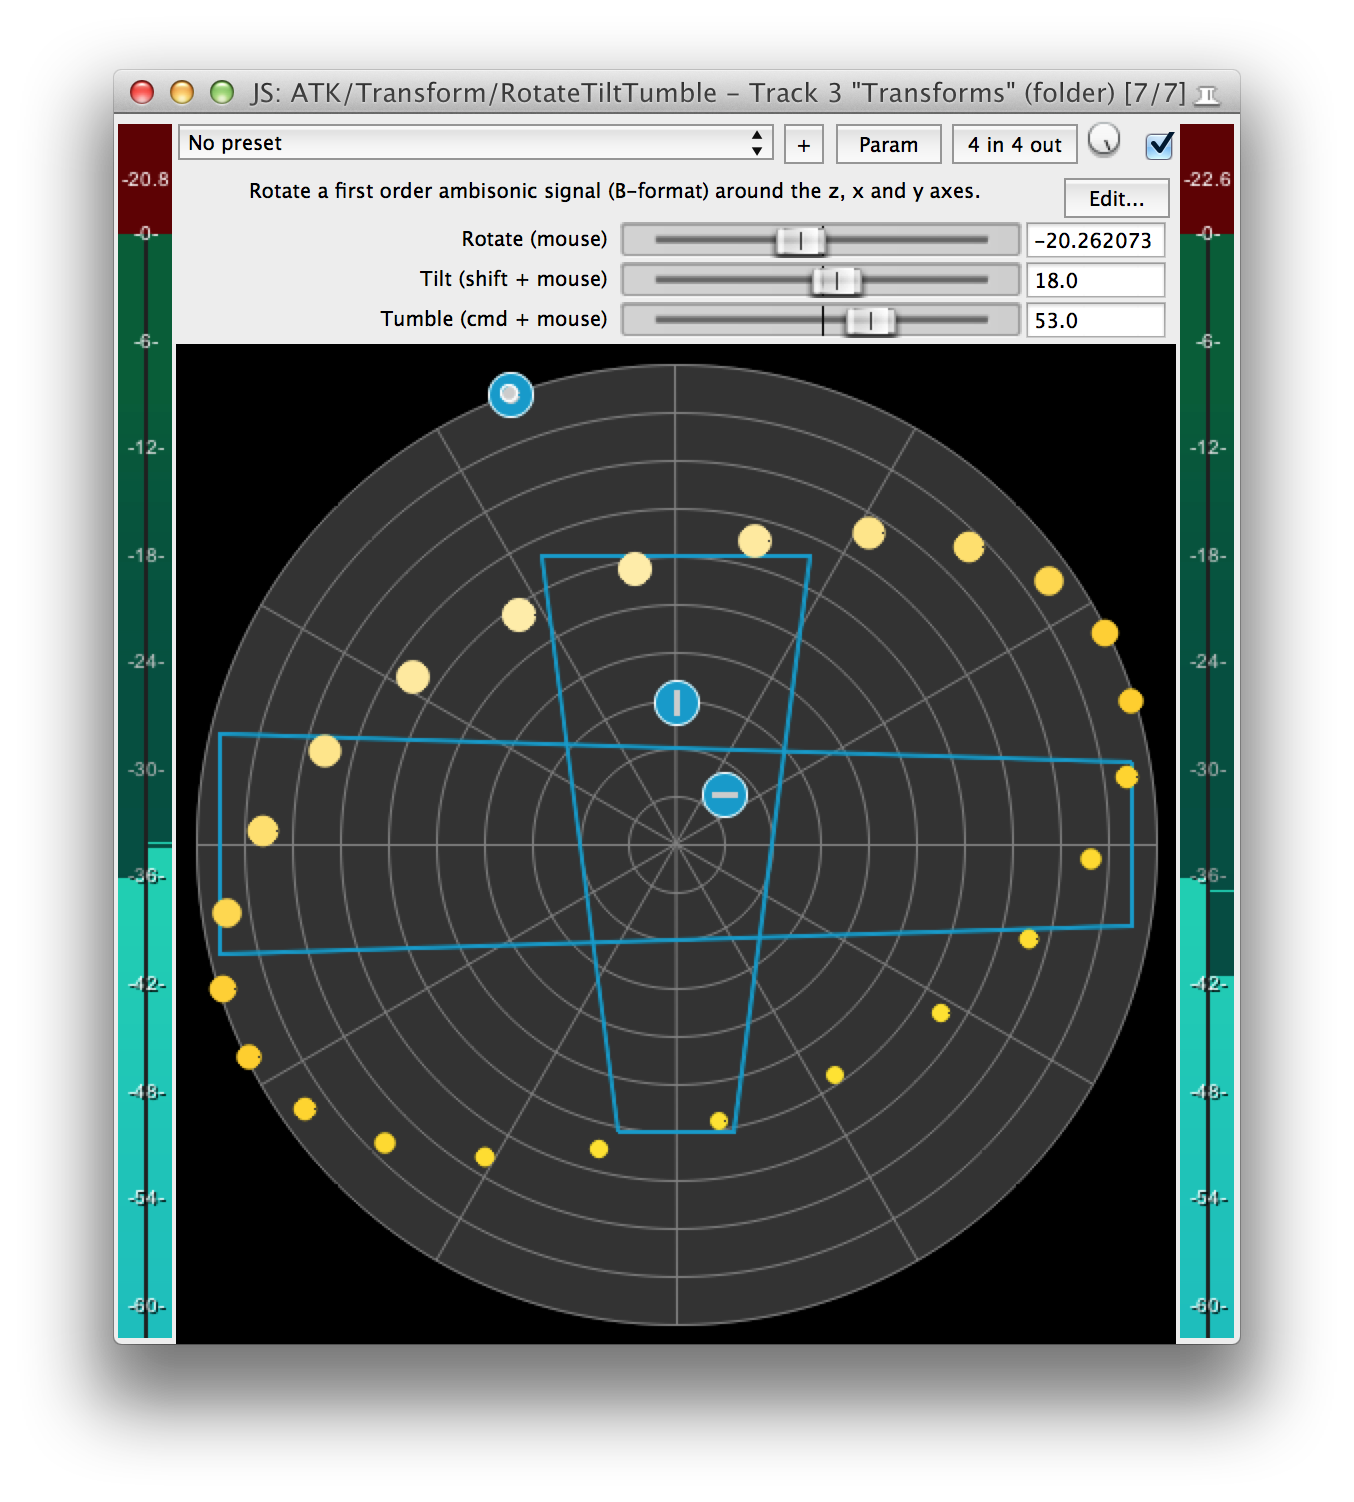
\includegraphics[width=0.9\columnwidth]{figures/rotateTiltTumble.png}
\setlength{\abovecaptionskip}{0pt plus 3pt minus 2pt} % Decrease distance, as the figure itself has lots of empty space below
\caption{Rotate, Tilt and Tumble transform.\label{fig:rotateTransform}}
\end{figure}

The \emph{RotateTiltTumble} plugin is a FOA multi-axes rotation transformer, with \emph{Rotation}, \emph{Tilt} and \emph{Tumble}\footnote{Yaw, Roll, and Pitch} transforms provided in the sequence indicated by the plugin name.
If the user wishes to change the order of transformations, it is possible to daisy-chain two or more instances of the plugin.
This transform does not affect directivity of the signal. The screenshot in figure \ref{fig:rotateTransform} demonstrates how variations in saturation, lightness and radius of the displayed transformed sources serve to illustrate their vertical position. The separate effect of the \emph{Tilt} and \emph{Tumble} transformations is indicated by the two blue planes in the interface.



\subsubsection{Direct and DirectO}\label{sec:direct}

\begin{figure}[h]
\captionsetup{aboveskip=-6pt}
\centering
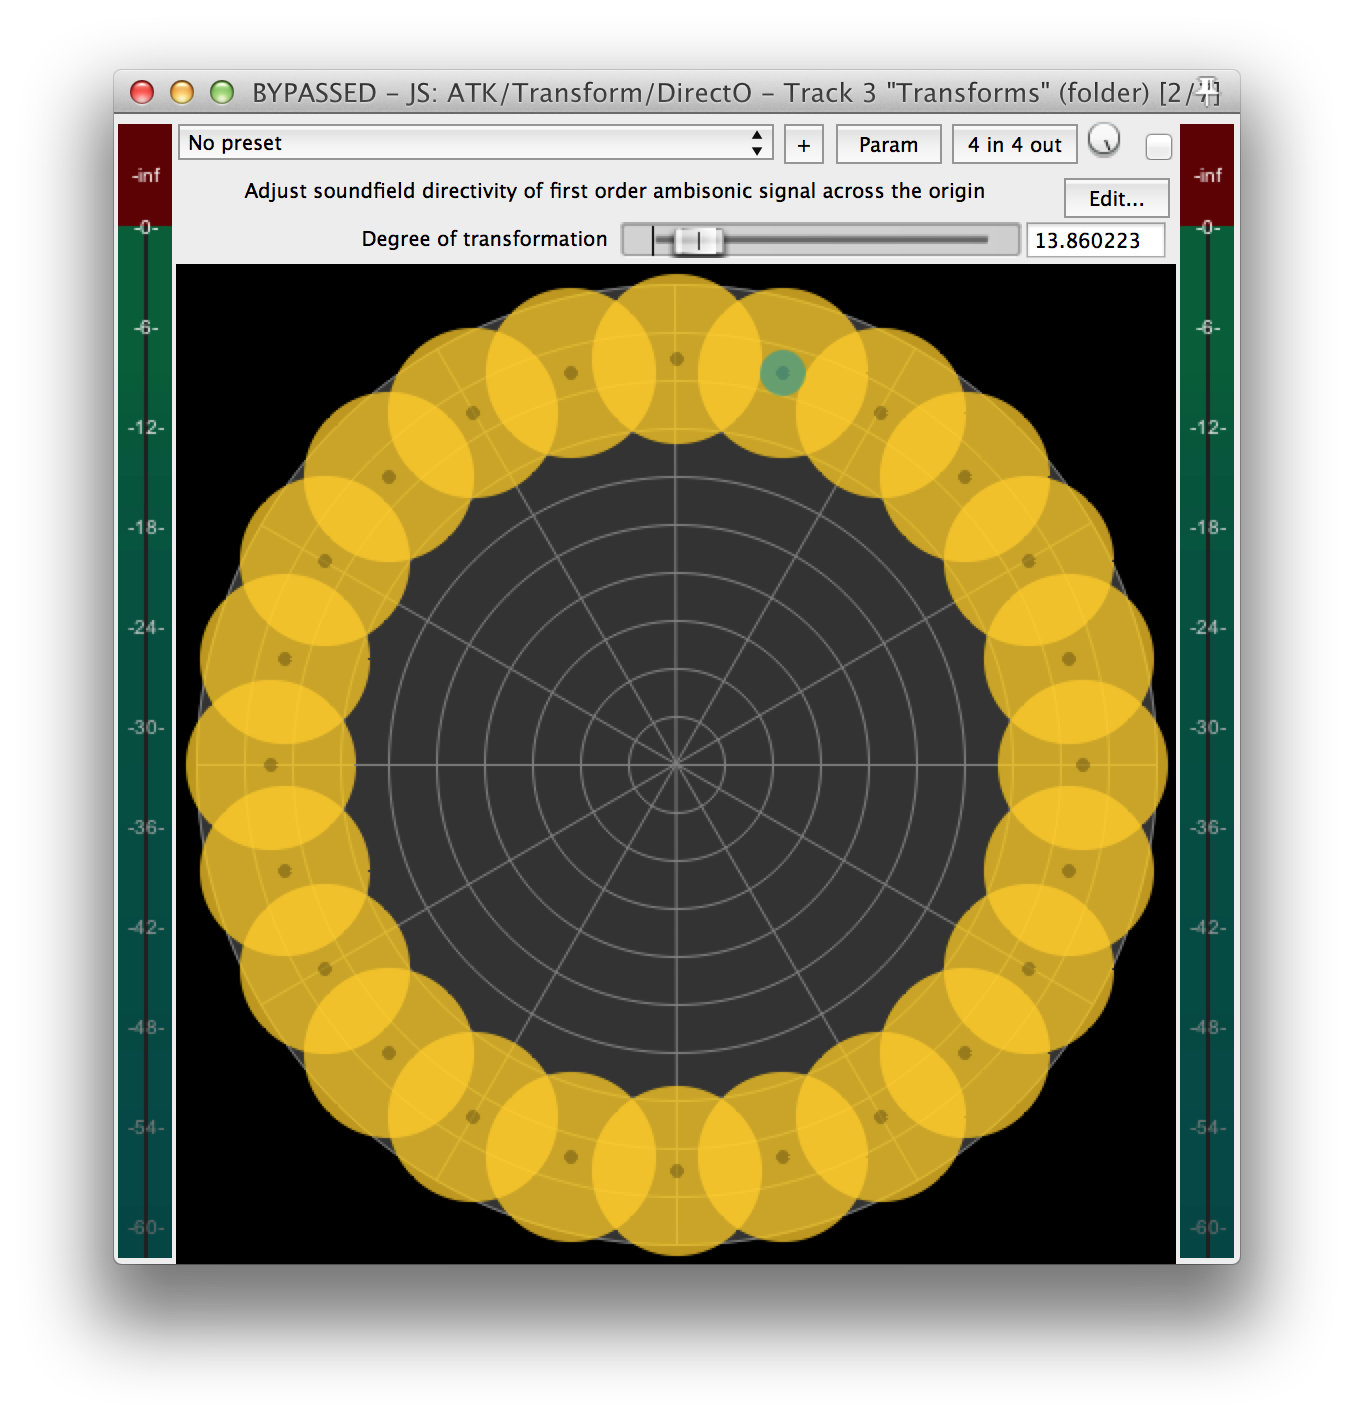
\includegraphics[width=0.9\columnwidth]{figures/directOTransform.png}
\caption{DirectO transform plugin interface.\label{fig:directOTransform}}
\end{figure}

The \emph{DirectO} plugin (figure \ref{fig:directOTransform}) adjusts the sound field directivity of a FOA signal across the origin.
It is a spatial low-pass filter; with increasing degree of transform, the signal becomes less directional, and with a transform of $90^{\circ}$ the signal becomes omnipresent.
  
\begin{figure}[h]
\captionsetup{aboveskip=-6pt}
\centering
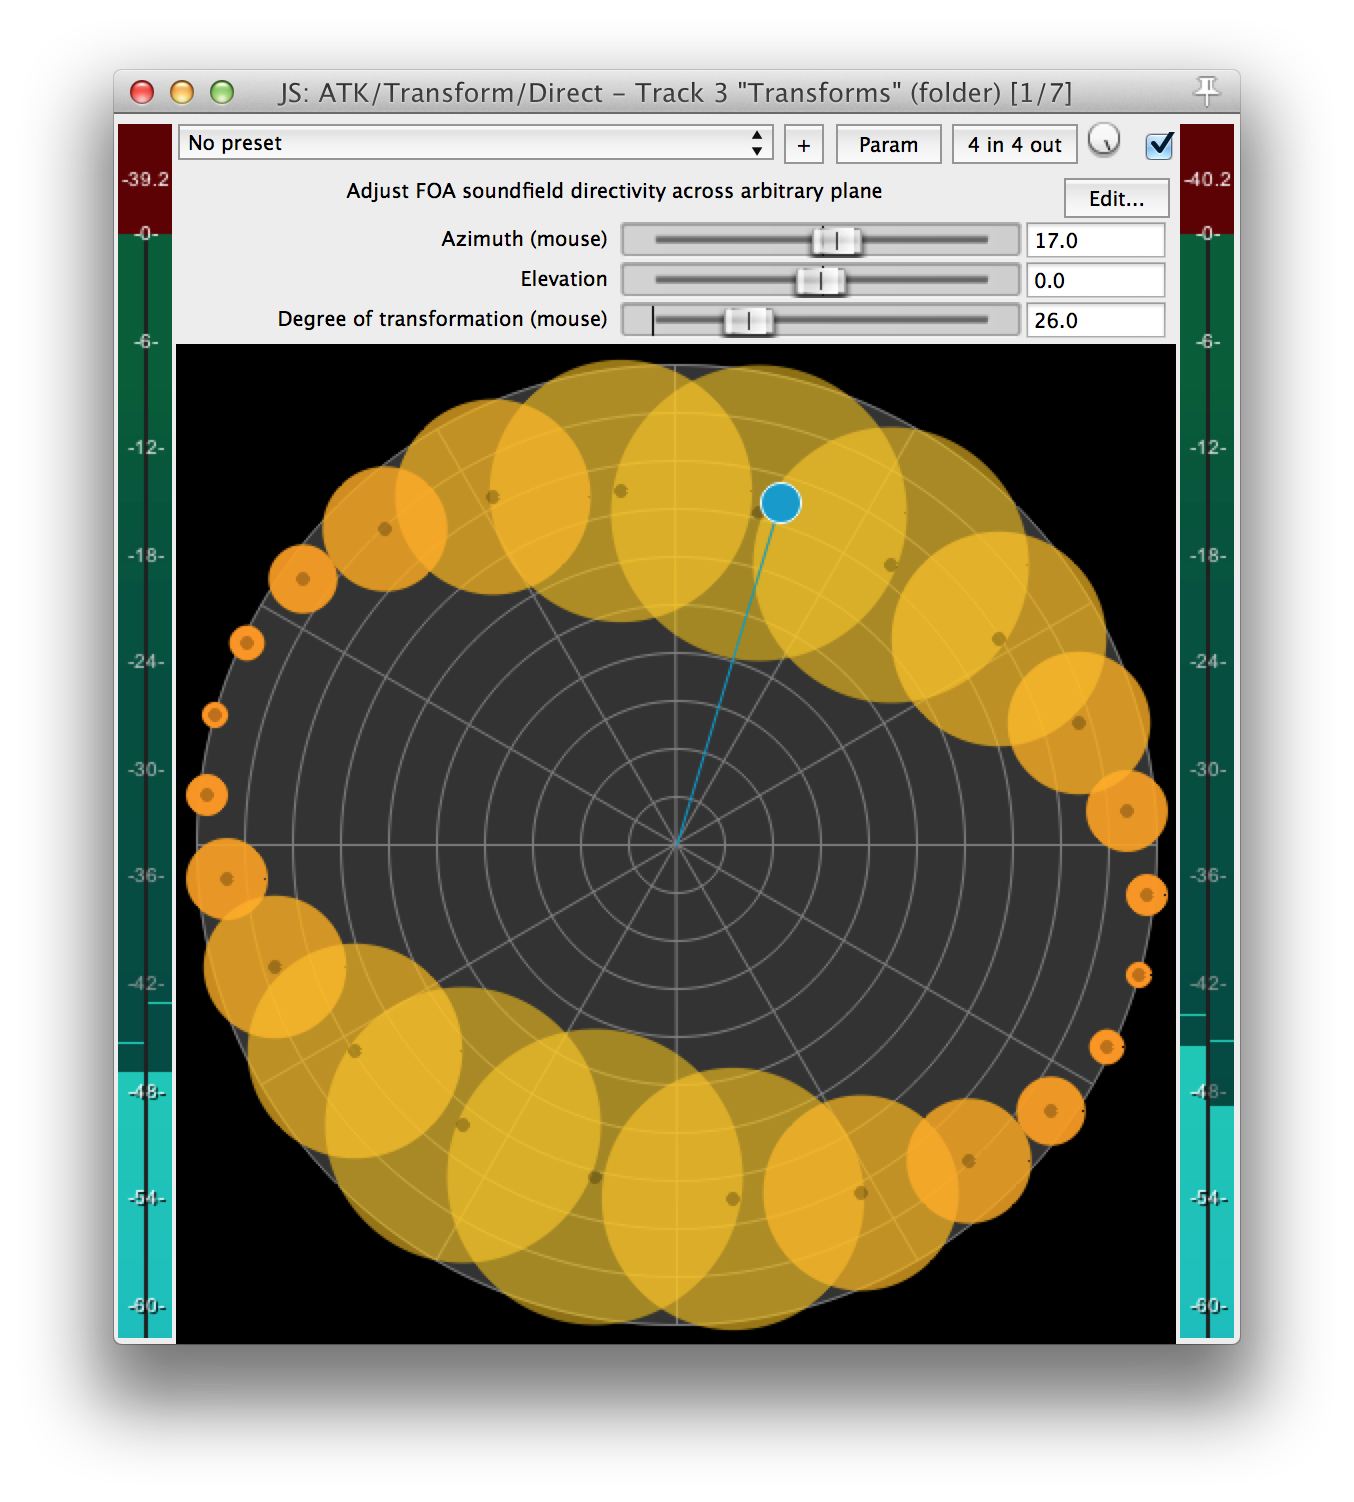
\includegraphics[width=0.9\columnwidth]{figures/directTransform.png}
\caption{Direct transform plugin interface.\label{fig:directTransform}}
\end{figure}

Similarly, the \emph{Direct} plugin (figure \ref{fig:directTransform}) adjusts the sound field directivity of a FOA signal across an arbitrary plane.


 
\subsubsection{FocusPushPressZoom and Dominate}\label{sec:focus}

\begin{figure}[h]
\captionsetup{aboveskip=-6pt}
\centering
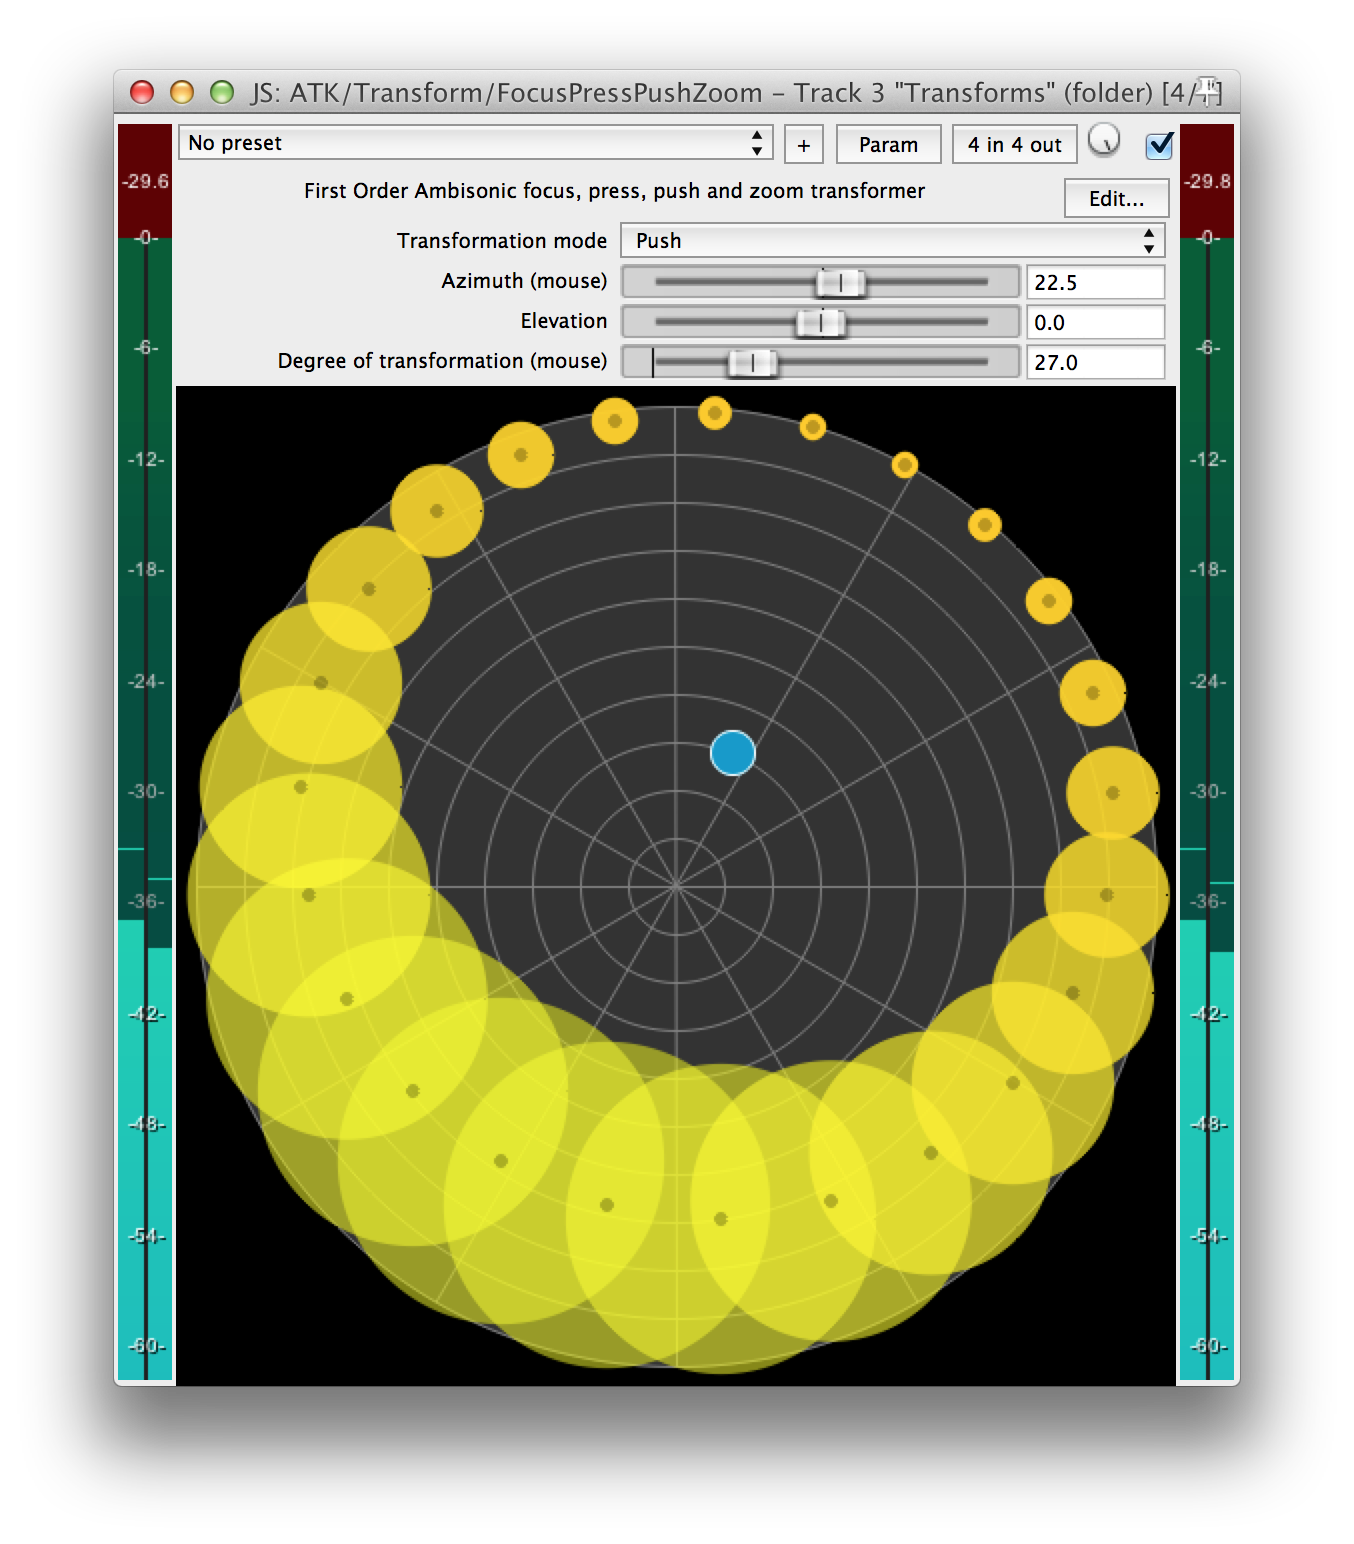
\includegraphics[width=0.9\columnwidth]{figures/pushTransform.png}
\setlength{\abovecaptionskip}{0pt plus 3pt minus 2pt} % Decrease distance, as the figure itself has lots of empty space below
\caption{Push transform plugin interface.\label{fig:pushTransform}}
\end{figure}

\begin{figure}[h]
\captionsetup{aboveskip=-6pt}
\centering
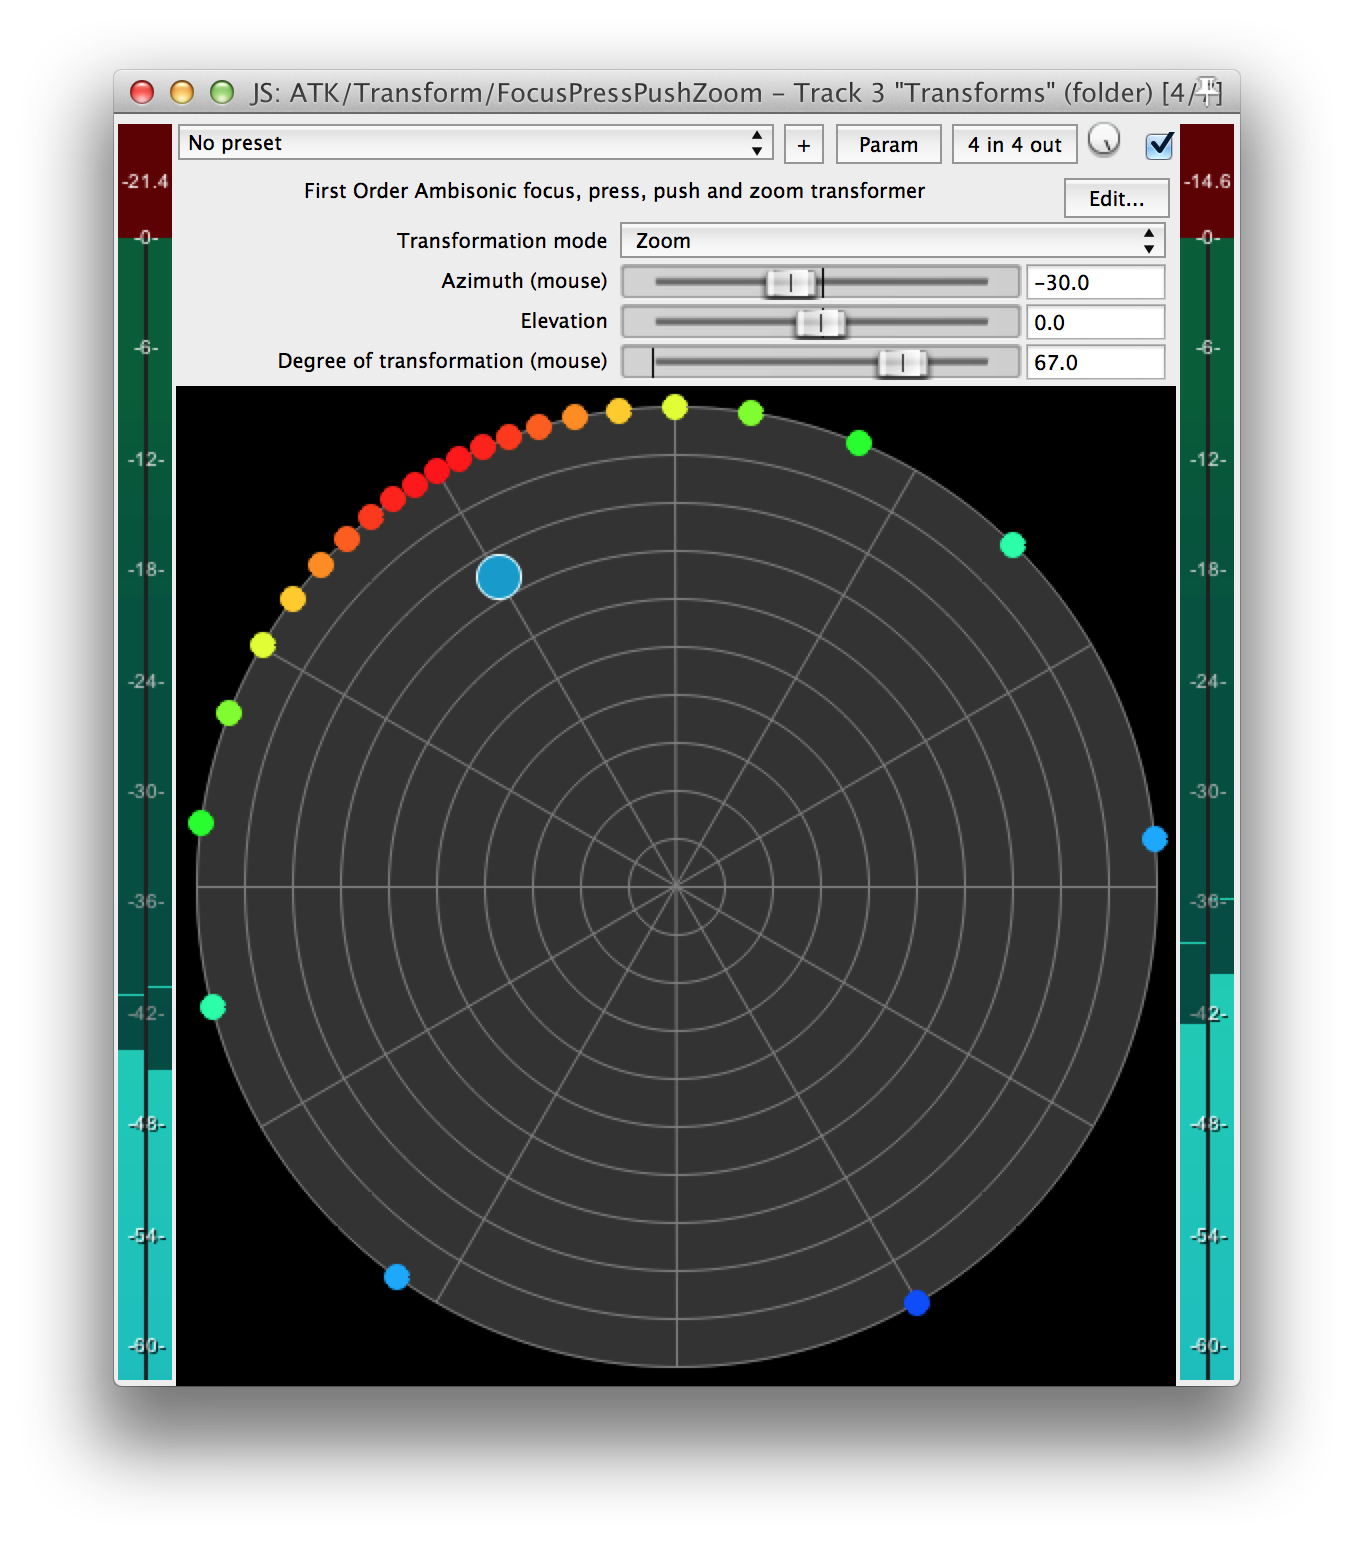
\includegraphics[width=0.9\columnwidth]{figures/zoomTransform.png}
\caption{Zoom transform interface.\label{fig:zoomTransform}}
\end{figure}

The \emph{FocusPushPressZoom} plugin provides a unified interface to the four different spatial transforms \emph{Focus}, \emph{Press}, \emph{Push} and \emph{Zoom}.
The degree of spatial transform is expressed as angles in the range from $0^\circ$ to $90^\circ$. 
At $0^\circ$ no transform is applied, while at $90^\circ$ all four transforms cause the soundfield to collapse to a single mono planewave.
%All four transforms shift the sound field in a preferred direction by altering directness, gain and direction of the incoming signals depending on their original directions, but the four transforms differ in terms of what mathematical transform is applied.
%The results will differ subtly or more distinctly depending on which of the transforms is applied.

The \emph{Focus} and \emph{Zoom} transforms are dominance related transforms and can be thought of as either `focusing' on or `emphasising' the elements of a soundfield in a certain direction. \emph{Focus} normalises the gain in the direction of interest to $0\,\mathrm{dB}$, where \emph{Zoom} normalises $\pm90^\circ$. At $180^\circ$ to the direction of interest both \emph{Focus} and \emph{Zoom} reduce the gain to $-\infty\,\mathrm{dB}$ when the transform angle is set to $\pm90^\circ$.

In contrast, \emph{Push} and \emph{Press} act differently, and rather than emphasising elements in a target direction, instead `push' all elements towards the direction of interest. When set to $\pm90^\circ$ the omnidirectional component of the soundfield (all elements) is transformed into a planewave arriving from the direction of interest.

%All four transforms shift the sound field in a preferred direction by altering directness, gain and direction of the incoming signals depending on their original directions, but the four transforms differ in terms of what mathematical transform is applied.
%The results will differ subtly or more distinctly depending on which of the transforms is applied.


Having all four transforms available in the same plugin makes this an expressive quality that can be explored in the creative process.
Two of the transforms can be seen in figures~\ref{fig:pushTransform} and \ref{fig:zoomTransform}.

The \emph{Dominance} plugin increases the gain of signals coming from the preferred direction while decreasing the gain of signals originating from the opposite side.
In the Reaper plugin gain in the preferred direction can be boosted by up to $24\,\mathrm{dB}$.
While the \emph{Focus}, \emph{Push}, \emph{Press}, and \emph{Zoom} transforms do not generally have any major impact on the overall sound level of the soundfield, \emph{Dominance} can result in major alterations to sound levels.
For this reason, as well as due to the difference in how the degree of transform is expressed (decibels rather than angles) the \emph{Dominance} transform has not been integrated into the same plugin as the other four transforms.


\subsubsection{Mirroring}\label{sec:mirror}

The \emph{Mirror} plugin mirrors the soundfield across an arbitrary plane, while the \emph{MirrorO} plugin mirrors the sound field across the origin.



\subsection{Near-field effects}\label{sec:near-field}

\emph{Proximity} facilitates the introduction of the proximity effect to encoded signals.
At extremes, the proximity effect introduces a strong bass boost, as well as phase differences.
The proximity effect can be an important contributor to perceptions of nearness.
Distance is described in meters, and to prevent bass boost from getting out of hand, the lower limit is set to $10\,\mathrm{cm}$ ($0.1\,\mathrm{m}$).

Near\-field compensation (NFC) is implemented via the \emph{NearFieldCompensation} plugin, and facilitates the reduction or removal of the proximity effect from encoded signals.
NFC is usually used in conjunction with decoders to compensate for the distance of loudspeakers on playback in loudspeaker rigs with smaller diameter. For the artist, NFC can also be used to reduce the proximity effect found in nearfield recordings.

\emph{Proximity} and \emph{NearFieldCompensation} respectively apply an integrator or high pass filter to the first order components of the encoded signal.\footnote{A 1\textsuperscript{th}-order high pass filter is the reciprocal of a 1\textsuperscript{th}-order integrator.} The \emph{Proximity} filter undoes \emph{NearFieldCompensation} given the same distance argument.


\subsection{Audio Effects and Ambisonics}\label{sec:a-format}

Spatial information is encoded in balance and phase relations between the four channels of a B-format signal.
Processing one or more of the channels using an audio effect which modifies gain and phase relations will most likely disrupt or otherwise distort the encoded spatial information. In most cases this is un-desired.

\begin{figure}[h]
\captionsetup{aboveskip=-6pt}
\centering
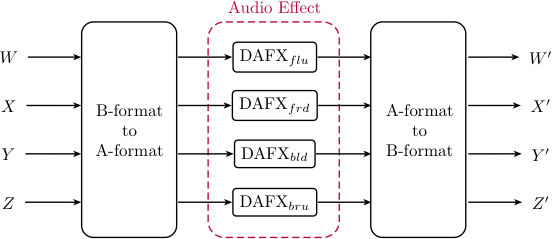
\includegraphics[width=1.0\columnwidth]{figures/DAFXNetwork.png}
\setlength{\abovecaptionskip}{0pt plus 3pt minus 2pt} % Decrease distance, as the figure itself has lots of empty space below
\caption{Process effects in A-format.\label{fig:aToB}}
\end{figure}

The ATK provides a remedy through the use of a pair of plugins, \emph{BtoA} and \emph{AtoB}, allowing the artist to process B-format signals using familiar audio effects. Figure~\ref{fig:aToB} illustrates the appropriate network. The \emph{BtoA} plugin decodes to A-format, while \emph{AtoB} re-encodes into B-format. When used in conjunction, the intermediate A-format signal is well-suited for effect processing. Spatial encoding is preserved (or modified) in a similar way as effects processing with two-channel stereo.

The \emph{Omni} mono signal encoder in conjunction with the network illustrated in figure~\ref{fig:aToB} can also be used to synth\-esise interesting soundfields. Each of the effects units should be tuned with slightly different parameters to ensure an active soundfield.
%On its own, \emph{AtoB} is often used to author immersive, periphonic (3D) decorrelated soundfields.


%Processed one or more of the channels using filters, distortion, delays, or some other audio effect, the spatial information of the encoded signal will most likely be distorted or otherwise lost, often resulting in distorted or unintended spatial results. This will tend to be the case if processing effects the individual B-format channels individually, i.e., if un-synced changes in gain or phase occur. 



\subsection{Decoders}\label{sec:decoders}

Perhaps one of the most celebrated aspects of the Ambisonic sound technique has been its design as a hierarchal reproduction system, able to target a number of varying loudspeaker arrays.
The ATK provides a wide palate of optimised decoders.

The \emph{Mono} virtual microphone decoder returns a single monophonic channel, and can be used to "listen in" to the soundfield at the specified azimuth and elevation.
The soundfield may be decoded to \emph{Stereo} using a pair of virtual microphones.
\emph{Quad} is an optimised quadraphonic decoder with variable loudspeaker angle, \emph{5.0} uses Bruce Wiggins optimised ITU 5.0 recorders \cite{wiggins:2003optimised}, \emph{Pantophonic} is a regular 2D polygon decoder and \emph{Periphonic} is a regular cylindrical decoder for 3D dual ring.
\emph{Diametric} is Gerzon's classic decoder suitable for varied periphonic and pantophonic loudspeaker arrays \cite{gerzon:1980sphere}.
While the regular decoders will be suitable for many users, diametric decoding enables the greatest flexibility, and allows the user to design substantially varying semi-regular arrays suitable for a wide variety of playback situations.
Meeting all the criteria outlined by Gerzon to qualify as Ambisonic, this decoder is a good choice for full 3D critical studio listening.

The \emph{UHJ} decoder and binaural decoders, using measured and synthetic HRTFs, requires kernel convolution, and remains to be implemented.
While the virtual microphone stereophonic decoder is very easy and convenient, for production work the authors advise using the \emph{UHJ} decoder, once the port has been accomplished.

The relevant decoders supports several decoding modes: 
The `dual' decoder is a dual-band psycho-acoustically optimised decoder, and the optimum choice for small scale studio or domestic settings \cite{heller:2008isAmbisonic}.
`single' is suitable for larger, mid-scale environments.
`velocity' returns `strict soundfield' (aka `basic') decoding, and is not preferred for First order Ambisonics in most circumstances.
`controlled' returns `controlled opposites' decoding (aka `in phase'), which is often preferred in large-scale, concert environments.


% DISCUSS: It would be useful to have some kind of visualisation of the speaker layout in a GUI in order to make it more intuitive to understand what the different layouts are?

% DISCUSS: IMHO the best thing would be to implement the shelf filter as a separate plugin, that is unless all of the decoders can be catered for in the same plugin. It's more DRY (don't repeat yourself) and also implies that the shelf filter is available for use in other contexts as well.





\subsection{Licensing and distribution}\label{sec:license}

ATK for SuperCollider3 is distributed as open-source using the GNU General Public License Version 3 (GNU GPL). This license is incompatible for use with proprietary software such as Reaper, and for this reason ATK for Reaper is distributed using the GNU Lesser Public License Version 3 (GNU LGPL).
ATK for Reaper requires Reaper 4.61 or newer, and will be available for download from the Ambisonic Toolkit web site in the near future \cite{ambisonictoolkit.net:2014}.



%%%%%%%%%%%%%%%%%%%%%%%%%%%%%%%%%%%%%%%%%%%%%%%%%%%%%%%%%%%%%%%%%%%%%%%%%%%%%
% Discussion
%%%%%%%%%%%%%%%%%%%%%%%%%%%%%%%%%%%%%%%%%%%%%%%%%%%%%%%%%%%%%%%%%%%%%%%%%%%%%
\section{Discussion}\label{sec:discussion}

While there is a well-established workflow for stereo on DAWs, options have been more limited when working with Ambisonics.
From a compositional viewpoint, Ambisonic field recordings sometimes can leave the sonic artist with an impression of `take it or leave it', as the sound image can be spectrally as well as spatially quite `full'.
In addition to rich sets of encoders and decoders, Ambisonic Toolkit offers intriguing possibilities for spatial transforms of the soundfield image, and for this reason it has been attractive to port ATK to a plugin format making it available in DAW workflows in addition to SuperCollider.
When porting ATK the prime question is whether to implement plugins in C++ using plugin architectures such as VST or AudioUnit.
If doing this, it seems beneficial to use a intermediate library such as Faust, Juce or wdl-ol, but it will still require substantial overhead in terms of having to compile and test the plugins for multiple processors and platforms.
At the same time the plugins are vulnerable to future changes in OS and plugin platforms.
At the end of 2013 Steinberg stopped maintenance and distribution of the VST2 SDK, instead requiring future developers to use VST3. The future of AudioUnit currently is somewhat uncertain, as the SDK has not been updated since 2007, and AU plugins can not be distributed via AppStore.

Reaper is a reasonably priced and flexible DAW for spatial sound, popular among many composers and sonic artists working with spatial sound, and provides the script-based language JSFX for plugins.
Using JSFX there is no need to compile, and plugins immediately work with all platforms and processors supported by Reaper.
As long as Reaper continues to be available, maintenance of the plugins are not expected to be demanding, as Reaper itself will take care of changes to e.g., operation systems.
Using JSFX has been speeding up the development process substantially, and development has been able to primarily focus only on the specific processing and interfacing.
One disadvantage is that graphics in plugins with custom GUIs seem to be demanding on system resources, and the program indicate major CPU overhead when plugin GUIs are open. However, once the GUI window is closed, the plugins do not seem to require any extraneous processing resources.




%%%%%%%%%%%%%%%%%%%%%%%%%%%%%%%%%%%%%%%%%%%%%%%%%%%%%%%%%%%%%%%%%%%%%%%%%%%%%
% Aknowledgments
%%%%%%%%%%%%%%%%%%%%%%%%%%%%%%%%%%%%%%%%%%%%%%%%%%%%%%%%%%%%%%%%%%%%%%%%%%%%%
\begin{acknowledgments}
Stian Remvik has provided valuable feedback on user interface design.
\end{acknowledgments} 

%%%%%%%%%%%%%%%%%%%%%%%%%%%%%%%%%%%%%%%%%%%%%%%%%%%%%%%%%%%%%%%%%%%%%%%%%%%%%
%bibliography here
\bibliography{2014-ICMC-ATK-Reaper}

\end{document}
